\documentclass[12pt, letterpaper]{article}

\usepackage[utf8]{inputenc}
\usepackage{booktabs}
\usepackage[table,xcdraw]{xcolor}
\usepackage{hyperref}
\hypersetup{
    colorlinks=true, %set true if you want colored links
    linktoc=all,     %set to all if you want both sections and subsections linked
    linkcolor=black,  %choose some color if you want links to stand out
}
\usepackage{graphicx}
\graphicspath{{./images/}}
\usepackage{float}

\usepackage[none]{hyphenat}

\tolerance=1
\emergencystretch=\maxdimen
\hyphenpenalty=10000
\hbadness=10000

\title{Sistema Gestione ZTL}
\author{Riccardo Maria Pesce}
\date{Anno Accademico 2019-2020}

\renewcommand{\contentsname}{Contenuti}

\begin{document}

\begin{titlepage}

\maketitle

\begin{abstract}

\noindent
In questa terza iterazione verrà eseguito un refactoring,
in modo da adempire ad alcuni pattern GRASP ed avere un 
software dove le componenti sono ulteriormente modulari.
In seguito, verrà complementata l'implementazione dei casi
d'uso \emph{UC3} ed \emph{UC4}

\end{abstract}
\end{titlepage}

\tableofcontents{}

\pagebreak

\section{Resoconto Iterazione 2}
Sebbene il sistema funzioni, si nota che esso 
è difficile da mantenere, dato che:
\begin{itemize}
    \item Il sistema centrale presenta un 
    antipattern, visto che si presenta 
    pieno di responsabilità
    \item Vengono passati parametri, anche 
    inutili, ai costruttori (esempio i costruttori
    \emph{Terminale} ed \emph{Autenticatore})
\end{itemize}

\noindent
Il programma sembra essere molto disordinato e 
disorganizzato, e questo non è una cosa positiva
nelle prossime fasi del progetto.

\noindent
Andiamo pertanto a definire il piano di questa 
iterazione.

\section{Piano per la Iterazione 3}
In questa terza iterazione implementeremo:
\begin{itemize}
    \item Il caso d'uso \emph{UC3}, includendo
    la funzione di rimozione del terminale.
    La funzione di modifica, dopo aver discusso,
    non verrà implementata in quanto essa consta 
    di due operazione (rimozione ed aggiunta) primitive
    gia implementate
    \item Il caso d'uso \emph{UC4}, includendo la 
    rimozione del residente. Per suddetti motivi,
    la modifica non verrà implementata
    \item Verranno implementati dei Controllori, per 
    accessi, in modo che vengano adempiti i pattern 
    \emph{GRASP Creator, Low Coupling, High Cohesion, 
    Expert,Controller}. Vedremo in seguito più 
    dettagli. Precisiamo che tale scelta influenzerà
    solamente la fase di progettazione e non analisi.
    \item Verrà eseguito un refactoring dei metodi/
    construttori.
\end{itemize}

\section{Requisiti}
\begin{itemize}
    \item L'impiegato deve poter registrare 
    un nuovo terminale, munito di codice 
    univoco, al sistema centrale il quale a 
    sua volta assegnerà al nuovo dispositivo 
    un profilo a seconda dei valichi e intervalli 
    consentiti.
    
    I profili che possono essere assegnati ad un 
    terminale sono due: 
    \begin{itemize}
        \item Il profilo abilitato a gestire i 
        residenti, i quali godono di accessi da 
        tutti i valichi ed intervalli illimitati.
        \item Il profilo abilitato a gestire gli 
        utenti carico-scarico, ossia gli utenti 
        abilitati all'accesso da un solo varco 
        in uno o due intervalli di tempo, della 
        durata di massimo un'ora.
    \end{itemize}
    Ogni terminale deve riconoscere tali tipologie 
    di utente per comportarsi adeguatamente.
    \item L'impiegato deve poter gestire 
    (aggiungere, rimuovere) la lista di utenti 
    residenti in modo tale che essi possano essere 
    gestiti correttamente dai terminali. 
    Tale lista sarà salvata in memoria persistente 
    a fine giornata e caricata dal sistema centrale 
    all'inizio del nuovo giorno.
\end{itemize}

\section{Modello dei Casi D'Uso}
Riportiamo i casi d'uso \emph{UC3} ed \emph{UC4}
nella loro completezza.

\subsection{Caso d'uso UC3 - Gestisci Terminale}

\emph{Attore primario: } Impiegato

\begin{itemize}
    \item \emph{Scenari principali di successo}
    \begin{itemize}
        \item \textbf{Aggiungi Terminale}
        \begin{enumerate}
            \item L'impiegato immette il codice 
            identificativo del terminale da 
            aggiungere.
            \item Il sistema, assicuratosi che tale 
            codice non appartenga ad altro terminale 
            installato, richiede all'impiegato il 
            profilo da associare al nuovo terminale.
            \item Si possono verificare le seguenti 
            opzioni:
            \begin{itemize}
                \item Il profilo richiesto è 
                \emph{carico-scarico}. In questo 
                caso, se non esiste un terminale 
                con tale profilo, la richiesta 
                viene accettata. Altrimenti, verrà 
                chiesto di modificare il profilo 
                dell'attuale terminale 
                \emph{carico-scarico} prima di 
                procedere. Questo perchè deve 
                essere solo uno il terminale 
                autorizzato al riconoscimento di 
                tale categoria di utenti. Di norma, 
                questo scenario dovrebbe avvenire 
                all'inizio, prima dell'avvio del 
                sistema, in quanto deve essere 
                garantito almeno un terminale con 
                questo profilo
                \item Il profilo richiesto è 
                \emph{residente}. In tal caso, dato 
                che non esistono limitazioni circa 
                tale categoria, il profilo viene 
                impostato correttamente e 
                nessun'altra azione è richiesta
            \end{itemize}
        \end{enumerate}
    \end{itemize}

    \begin{itemize}
        \item \textbf{Rimuovi Terminale}
        \begin{enumerate}
            \item L'impiegato immette il codice 
            identificativo del terminale da 
            rimuovere.
            \item Il sistema, assicuratosi che tale 
            esista, compie una delle seguenti azioni.
            \begin{itemize}
                \item Se il terminale da rimuovere 
                è di tipo \emph{carico-scarico}, 
                viene chiesto all'impiegato di 
                selezionare un altro terminale per 
                tale funzione.
                \item Se il terminale da rimuovere 
                ha profilo \emph{residente}, viene 
                rimosso semplicemnte, senza 
                ulteriori azioni.
            \end{itemize}
        \end{enumerate}
    \end{itemize}
\end{itemize}

\begin{itemize}
    \item \emph{Scenari alternativi}
    \begin{itemize}
        \item \textbf{Aggiungi Terminale}
        \begin{enumerate}
            \item Se il numero inserito è gia 
            presente, allora il sistema ritornerà 
            un messaggio d'errore.
            \item Se, nel caso in cui si sta 
            aggiungendo un terminale 
            \emph{carico-scarico} e quando viene 
            chiesto di cambiare il corrente 
            terminale designato a tale funzione, 
            viene fornita una risposta non 
            affermativa o sbagliata, il sistema 
            ritorna un messaggio d'errore.
        \end{enumerate}
    \end{itemize}

    \begin{itemize}
        \item \textbf{Rimuovi Terminale}
        \begin{enumerate}
            \item Se il codice identificativo non 
            esiste, viene ritornato un messaggio 
            d'errore.
            \item Se tale è l'unico terminale 
            attivo nel sistema, viene respinta la 
            richiesta con un apposito messaggio 
            d'errore.
            \item Se, nel caso in cui si vuole 
            rimuovere il terminale 
            \emph{carico-scarico}, 
            ed alla richiesta di inserire il codice 
            di un altro terminale per trasferire 
            tale profilo viene inserito un codice 
            inesistente, viene restituito un 
            messaggio d'errore e terminata 
            l'esecuzione.
        \end{enumerate}
    \end{itemize}
\end{itemize}


\subsection{Caso d'uso UC4 - Gestisci Residente}

\emph{Attore primario: } Impiegato

\begin{itemize}
    \item \emph{Scenari principali di successo}
    \begin{itemize}
        \item \textbf{Aggiungi Residente}
        \begin{enumerate}
            \item L'impiegato immette i dati 
            anagrafici, ed assegna al residente 
            il codice identificativo del 
            dispositivo telepass posseduto 
            dall'utente stesso.
            \item Il sistema, assicuratosi che 
            l'utente non esiste gia (attraverso 
            il controllo del codice identificativo), 
            lo registrerà con successo.
        \end{enumerate}

        \item \textbf{Rimuovi Residente}
        \begin{enumerate}
            \item L'impiegato immette il codice 
            identificativo dell'utente da rimuovere.
            \item Il sistema, assicuratosi che 
            l'utente esista, lo rimuove senza 
            ulteriori azioni.
        \end{enumerate}
    \end{itemize}

    \item \emph{Scenari alternativi}
    \begin{enumerate}
        \item \textbf{Aggiungi Residente}
        \begin{enumerate}
            \item Se l'utente gia esiste, 
            la richiesta verrà semplicemnte 
            ignorata con un messaggio d'errore.
        \end{enumerate}

        \item \textbf{Rimuovi Residente}
        \begin{enumerate}
            \item Se l'utente non esiste, 
            la richiesta verrà semplicemnte 
            ignorata con un messaggio d'errore.
        \end{enumerate}
    \end{enumerate}
\end{itemize}

\section{Modello di Dominio}
L'analisi di dominio identifica le classi 
concettuali identificate nella precedente
iterazione. 
\begin{figure}[H]
    \centering
    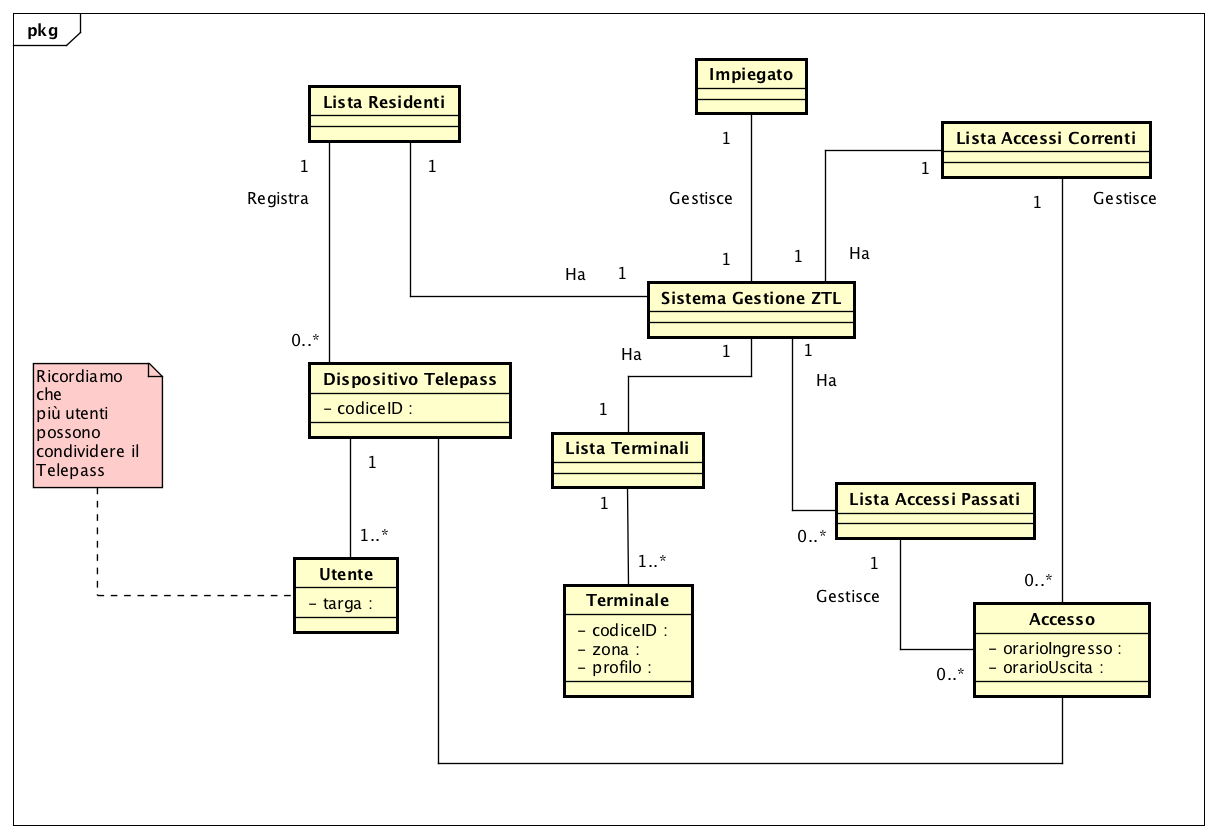
\includegraphics[scale=0.40]{ModelloDominio}
    \label{fig:mesh1}
\end{figure}

\section{Diagrammi di Sequenza di Sistema}

\subsection{UC3.2 \emph{(Rimuovi Terminale)}}
Dato che implementeremo due varianti
dell'operazione \texttt{rimuoviTerminale}
(in quanto si può rimuovere sia per id che 
per zona), nel diagramma si omettono 
volutamente i parametri.
\begin{figure}[H]
    \centering
    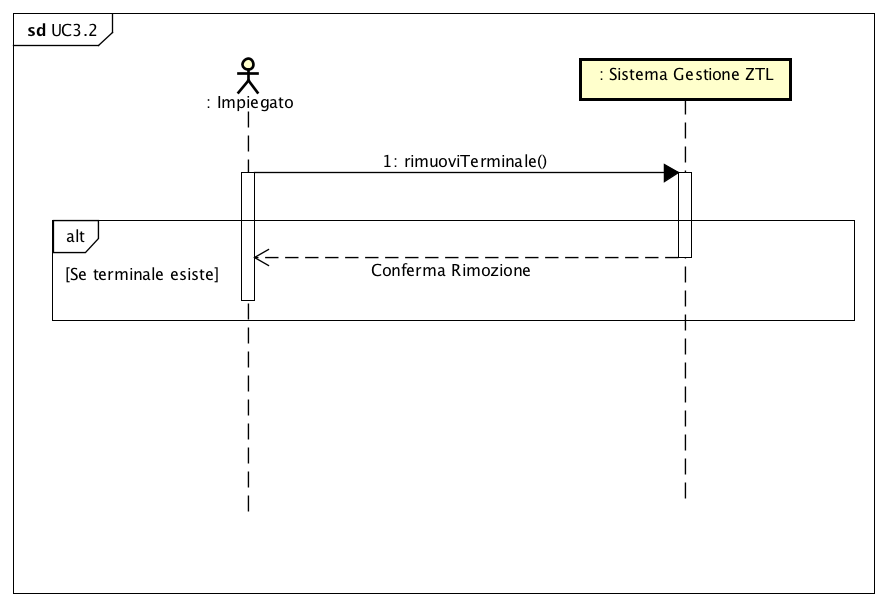
\includegraphics[scale=0.40]{UC3.2-SSD}
    \label{fig:mesh1}
\end{figure}

\subsection{UC4.2 \emph{(Rimuovi Residente)}}
\begin{figure}[H]
    \centering
    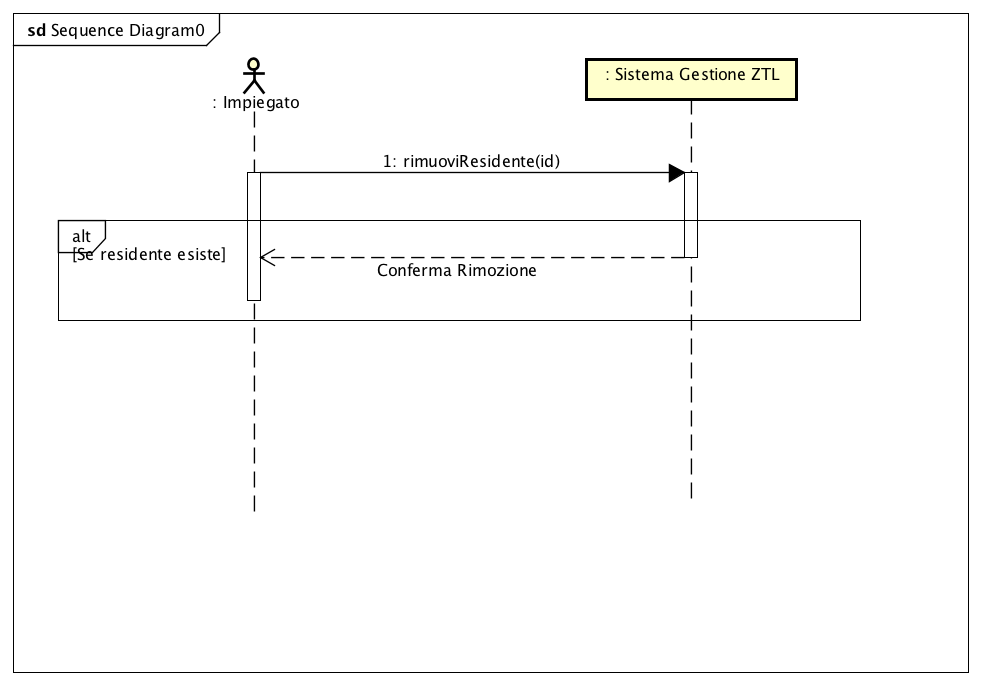
\includegraphics[scale=0.40]{UC4.2-SSD}
    \label{fig:mesh1}
\end{figure}

\section{Diagrammi di Interazione}
Innanzitutto riportiamo i diagrammi di 
interazione dei casi d'uso introdotti in 
questa iterazione, ed in seguito vogliamo 
riportare anche i diagrammi dei casi 
d'uso definiti in precedenza, rifiniti,
in modo da portarci al refactoring in 
maniera più agevole.

\subsection{UC3.2 - Rimuovi Terminale}
Nel caso in cui vogliamo rimuovere il 
terminale per \emph{id}, il diagramma 
si presenta così:
\begin{figure}[H]
    \centering
    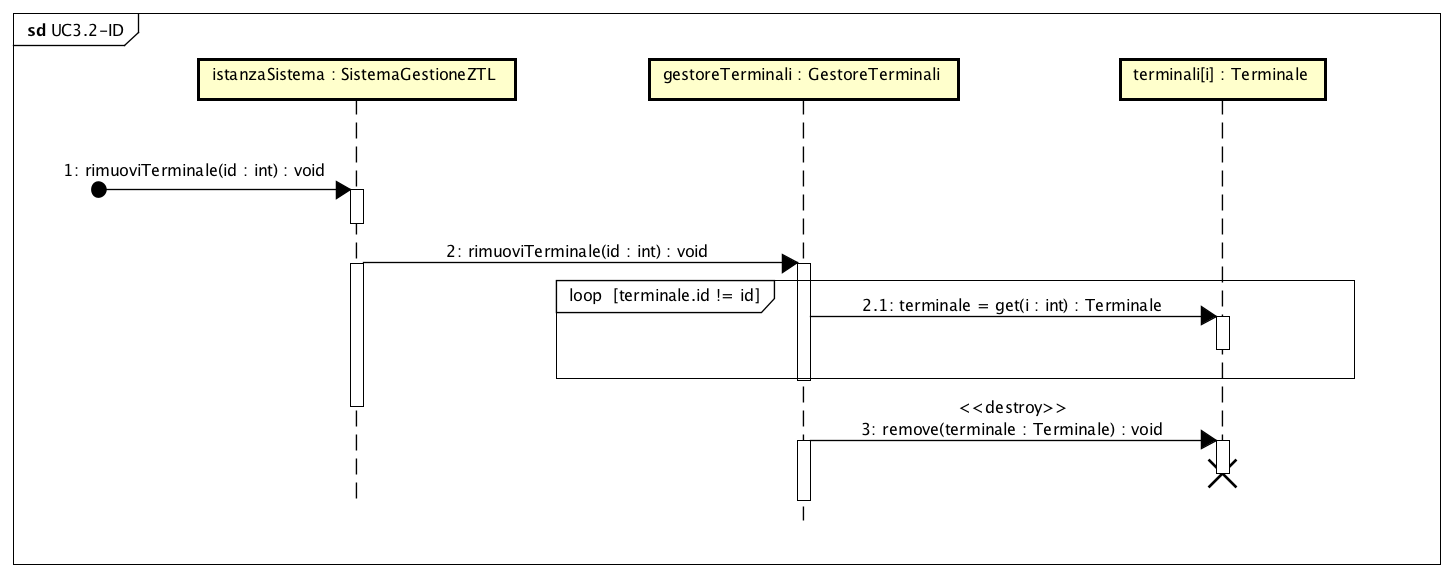
\includegraphics[scale=0.30]{UC3.2-DI-ID}
    \label{fig:mesh1}
\end{figure}

\noindent
Mentre se vogliamo rimuovere il terminale
per zona:
\begin{figure}[H]
    \centering
    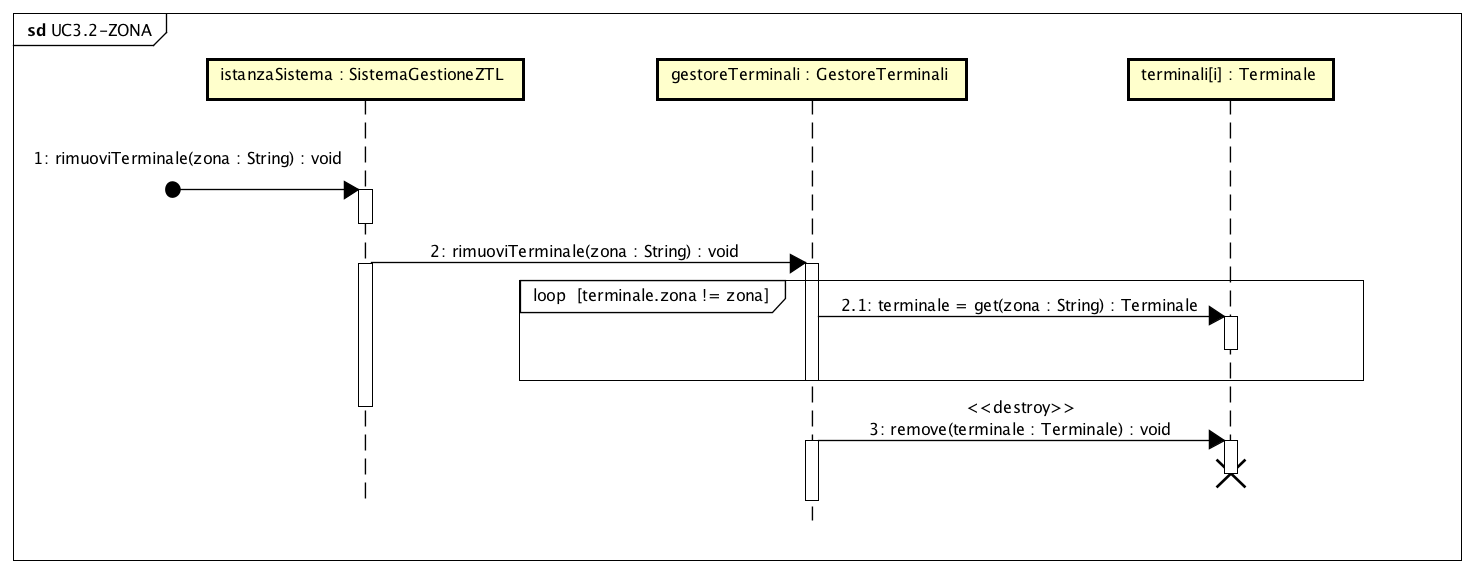
\includegraphics[scale=0.30]{UC3.2-DI-ZONA}
    \label{fig:mesh1}
\end{figure}

\subsection{UC4.2 - Rimuovi Residente}
\begin{figure}[H]
    \centering
    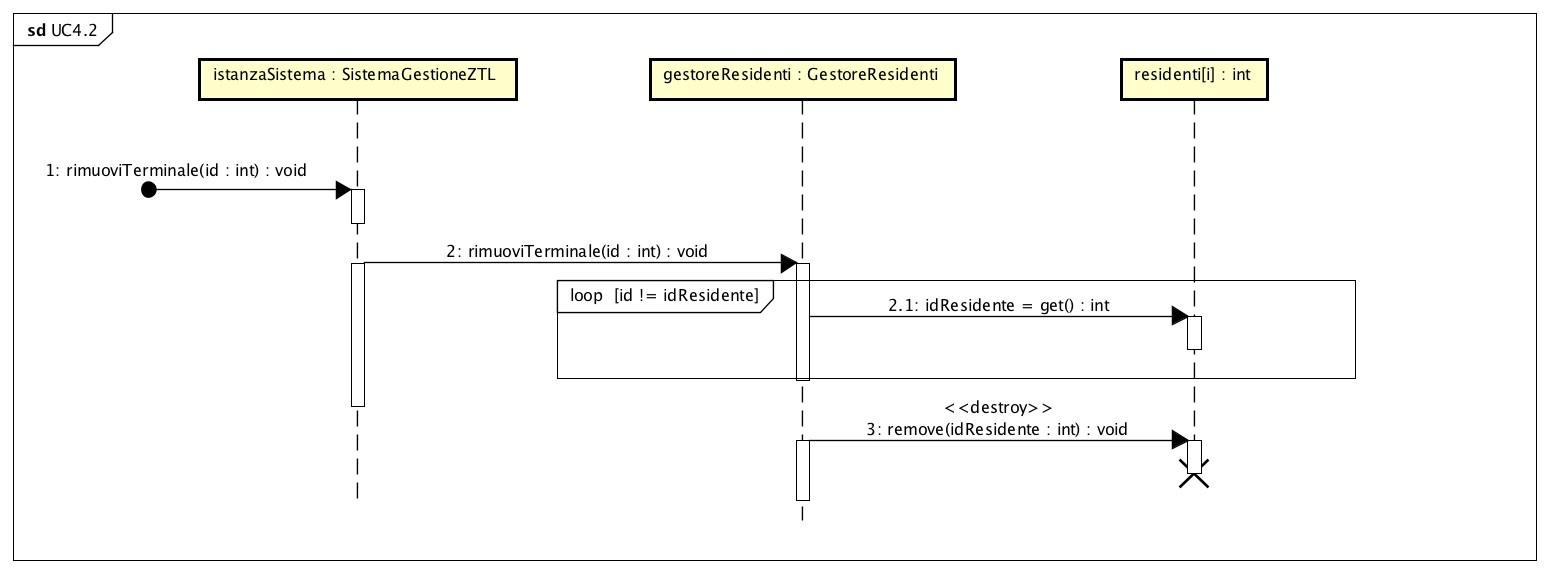
\includegraphics[scale=0.30]{UC4.2-DI}
    \label{fig:mesh1}
\end{figure}

\section{Diagrammi di Interazione refactored}
Questi diagrammi afferiscono alla precedente
iterazione, con le opportune modifiche apportate 
in tale iterazione.
\subsection{UC1}
\begin{figure}[H]
    \centering
    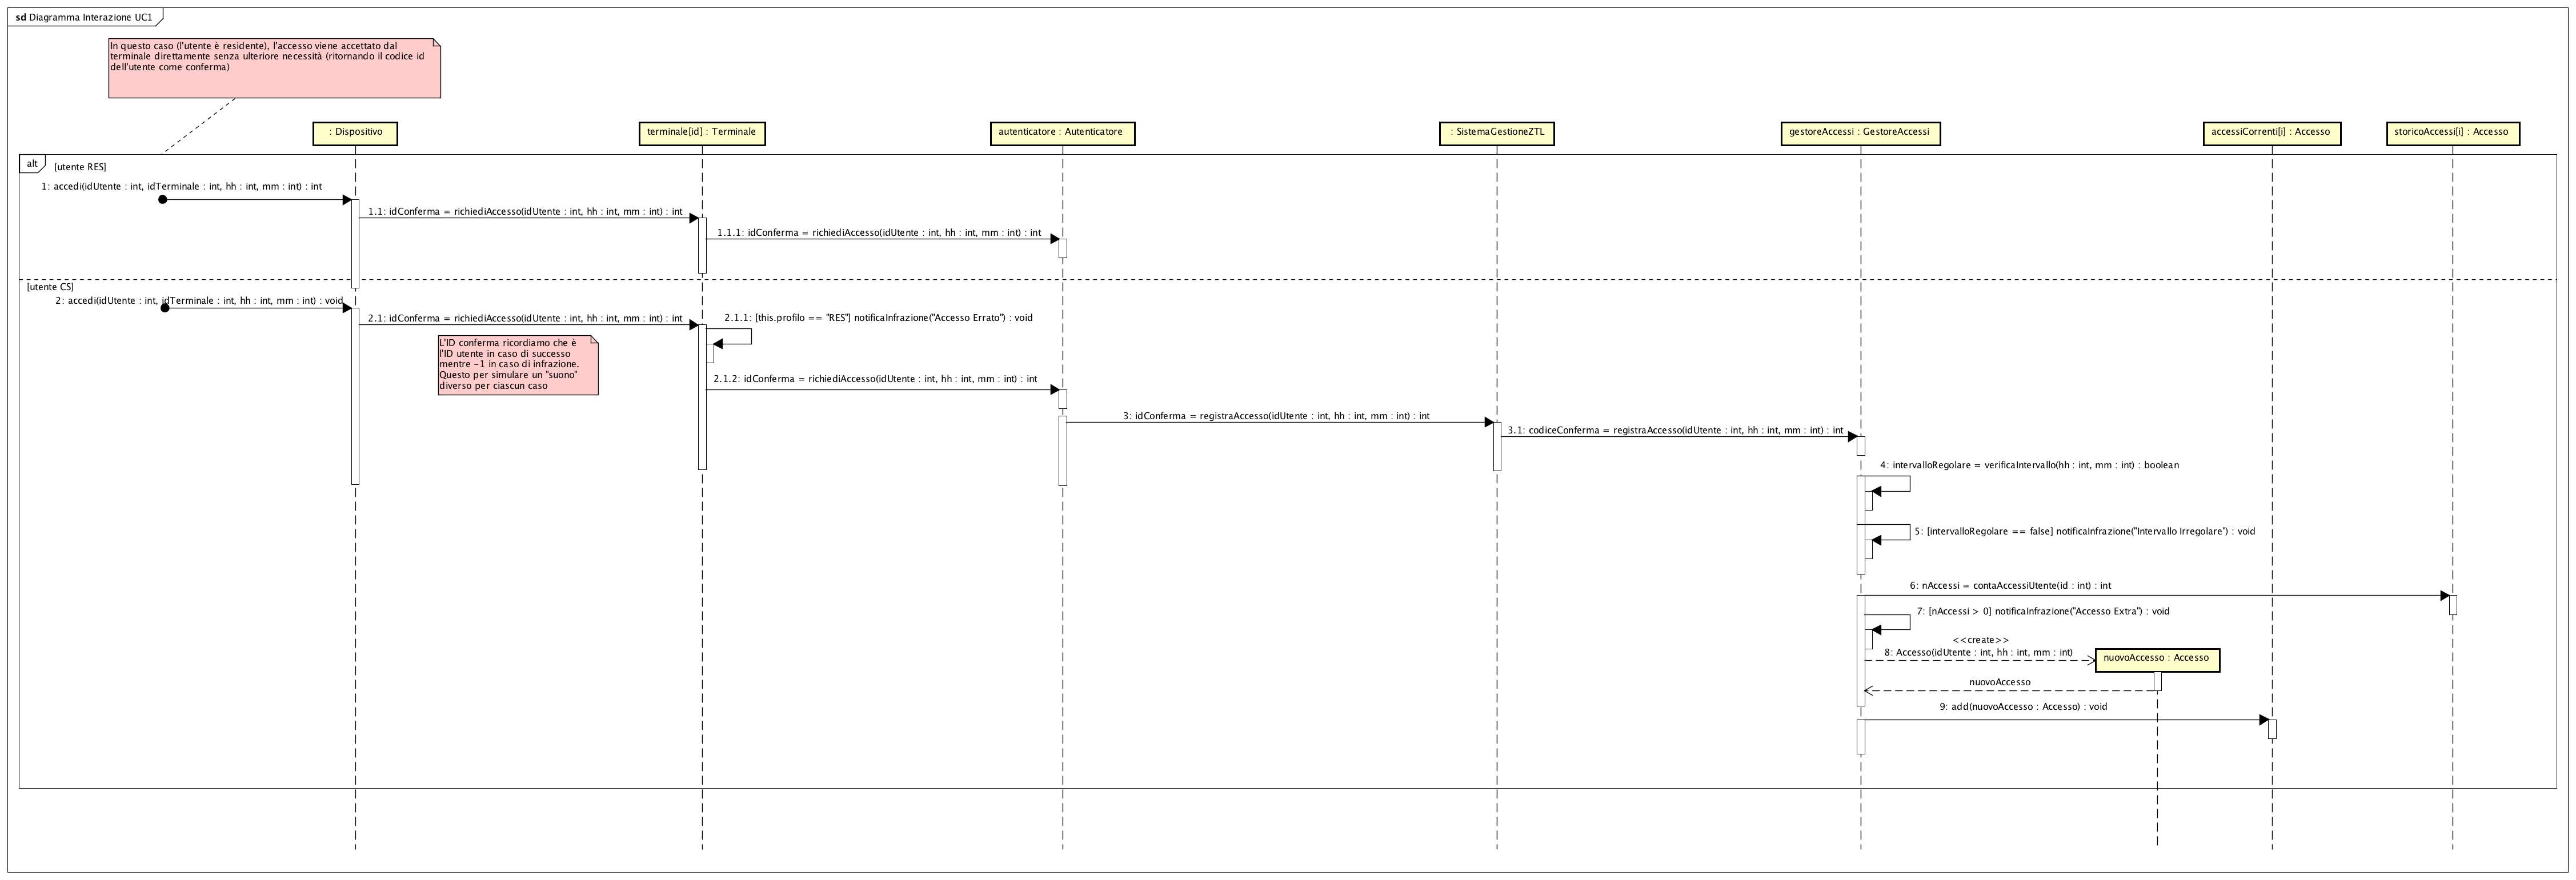
\includegraphics[scale=0.10]{UC1-DI}
    \label{fig:mesh1}
\end{figure}

\subsection{UC2}
\begin{figure}[H]
    \centering
    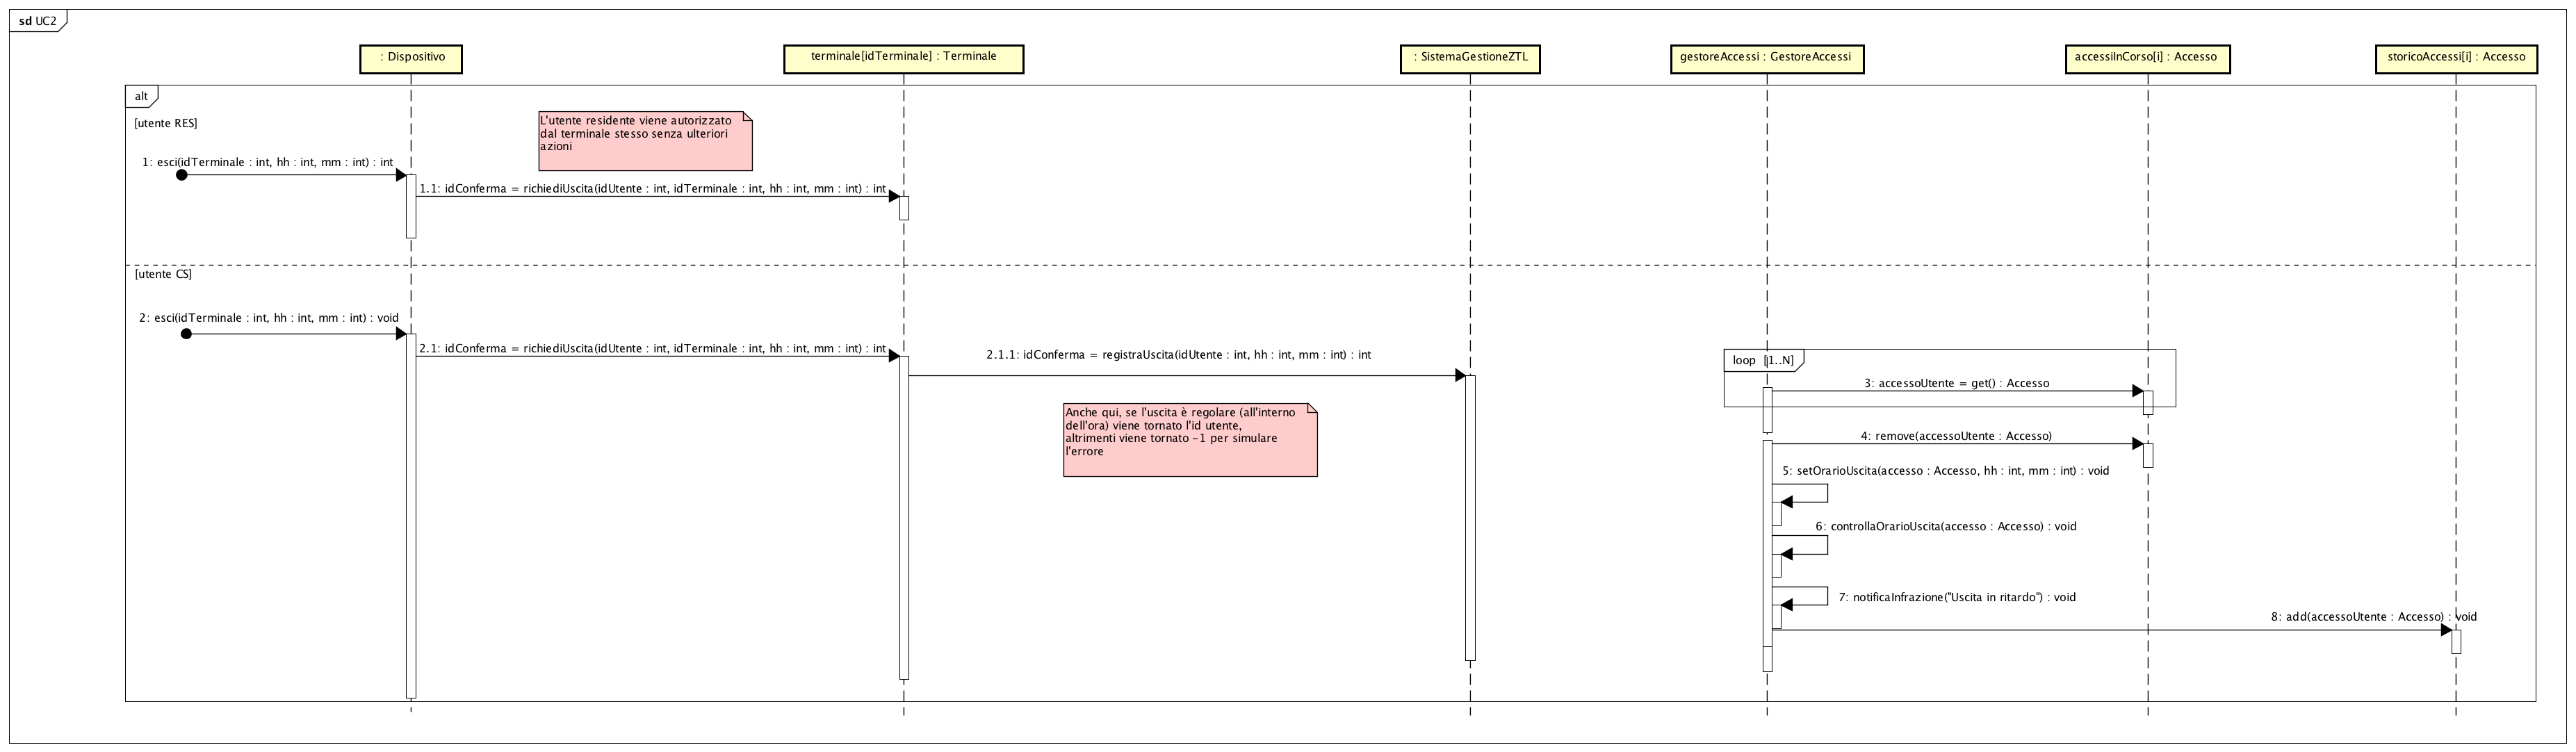
\includegraphics[scale=0.10]{UC2-DI}
    \label{fig:mesh1}
\end{figure}

\subsection{UC3.1 \emph{Aggiungi Terminale}}
\begin{figure}[H]
    \centering
    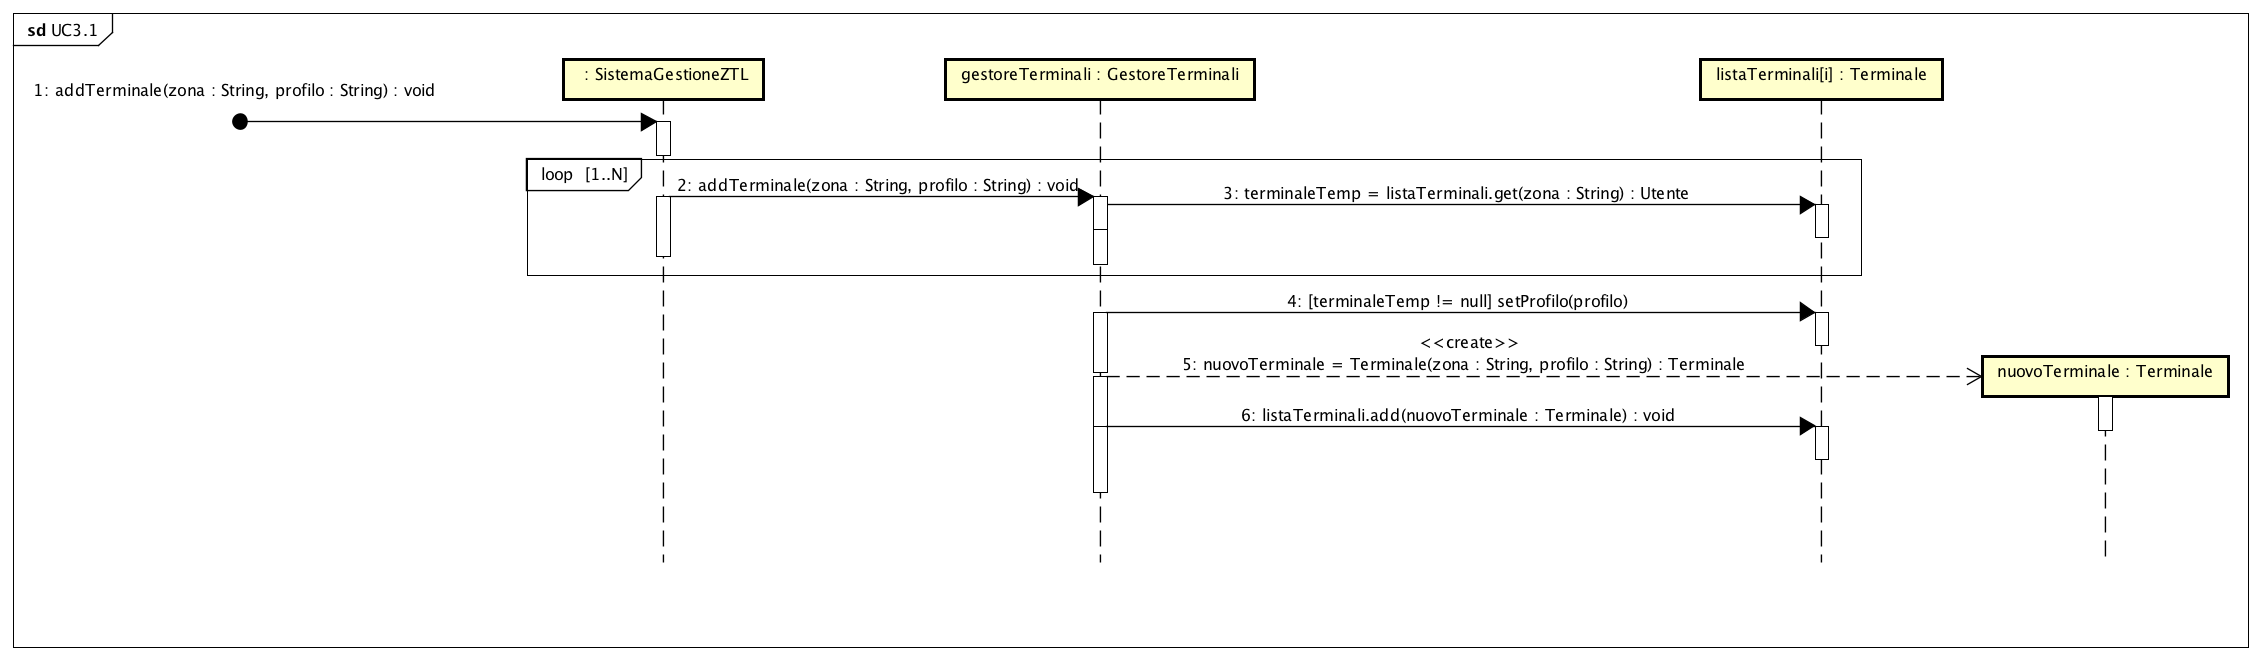
\includegraphics[scale=0.20]{UC3.1-DI}
    \label{fig:mesh1}
\end{figure}

\subsection{UC4.1 \emph{Aggiungi Residente}}
\begin{figure}[H]
    \centering
    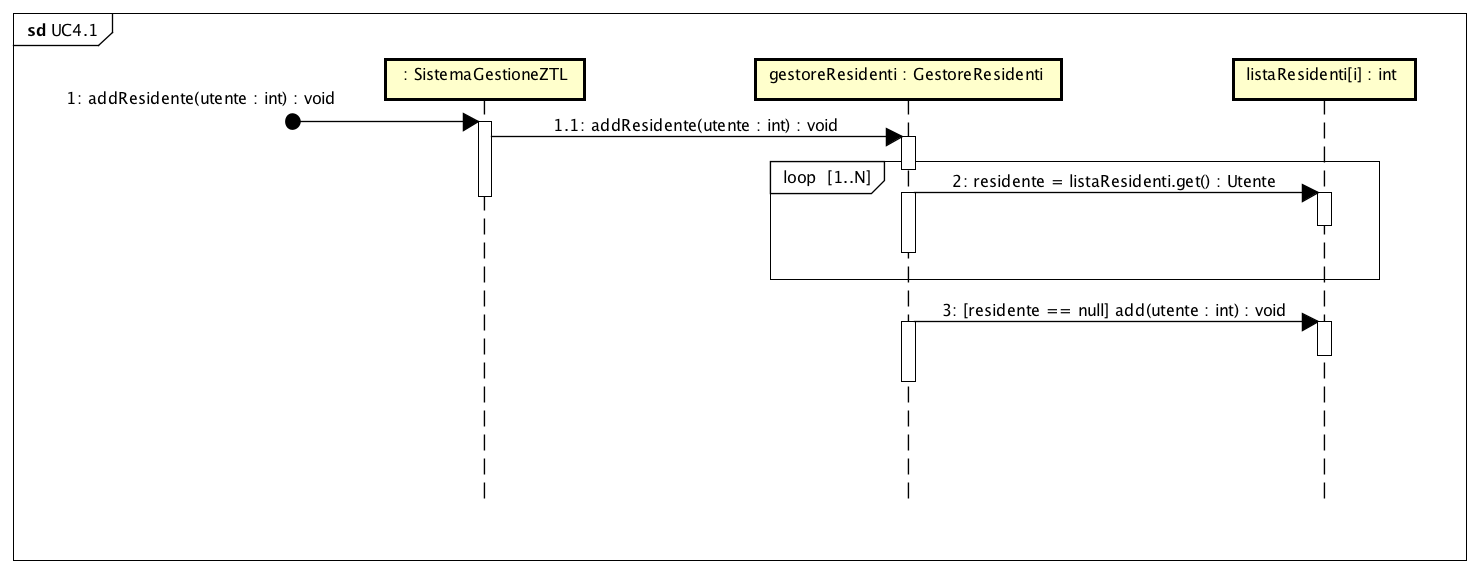
\includegraphics[scale=0.30]{UC4.1-DI}
    \label{fig:mesh1}
\end{figure}

\section{Diagramma delle Classi}
\begin{figure}[H]
    \centering
    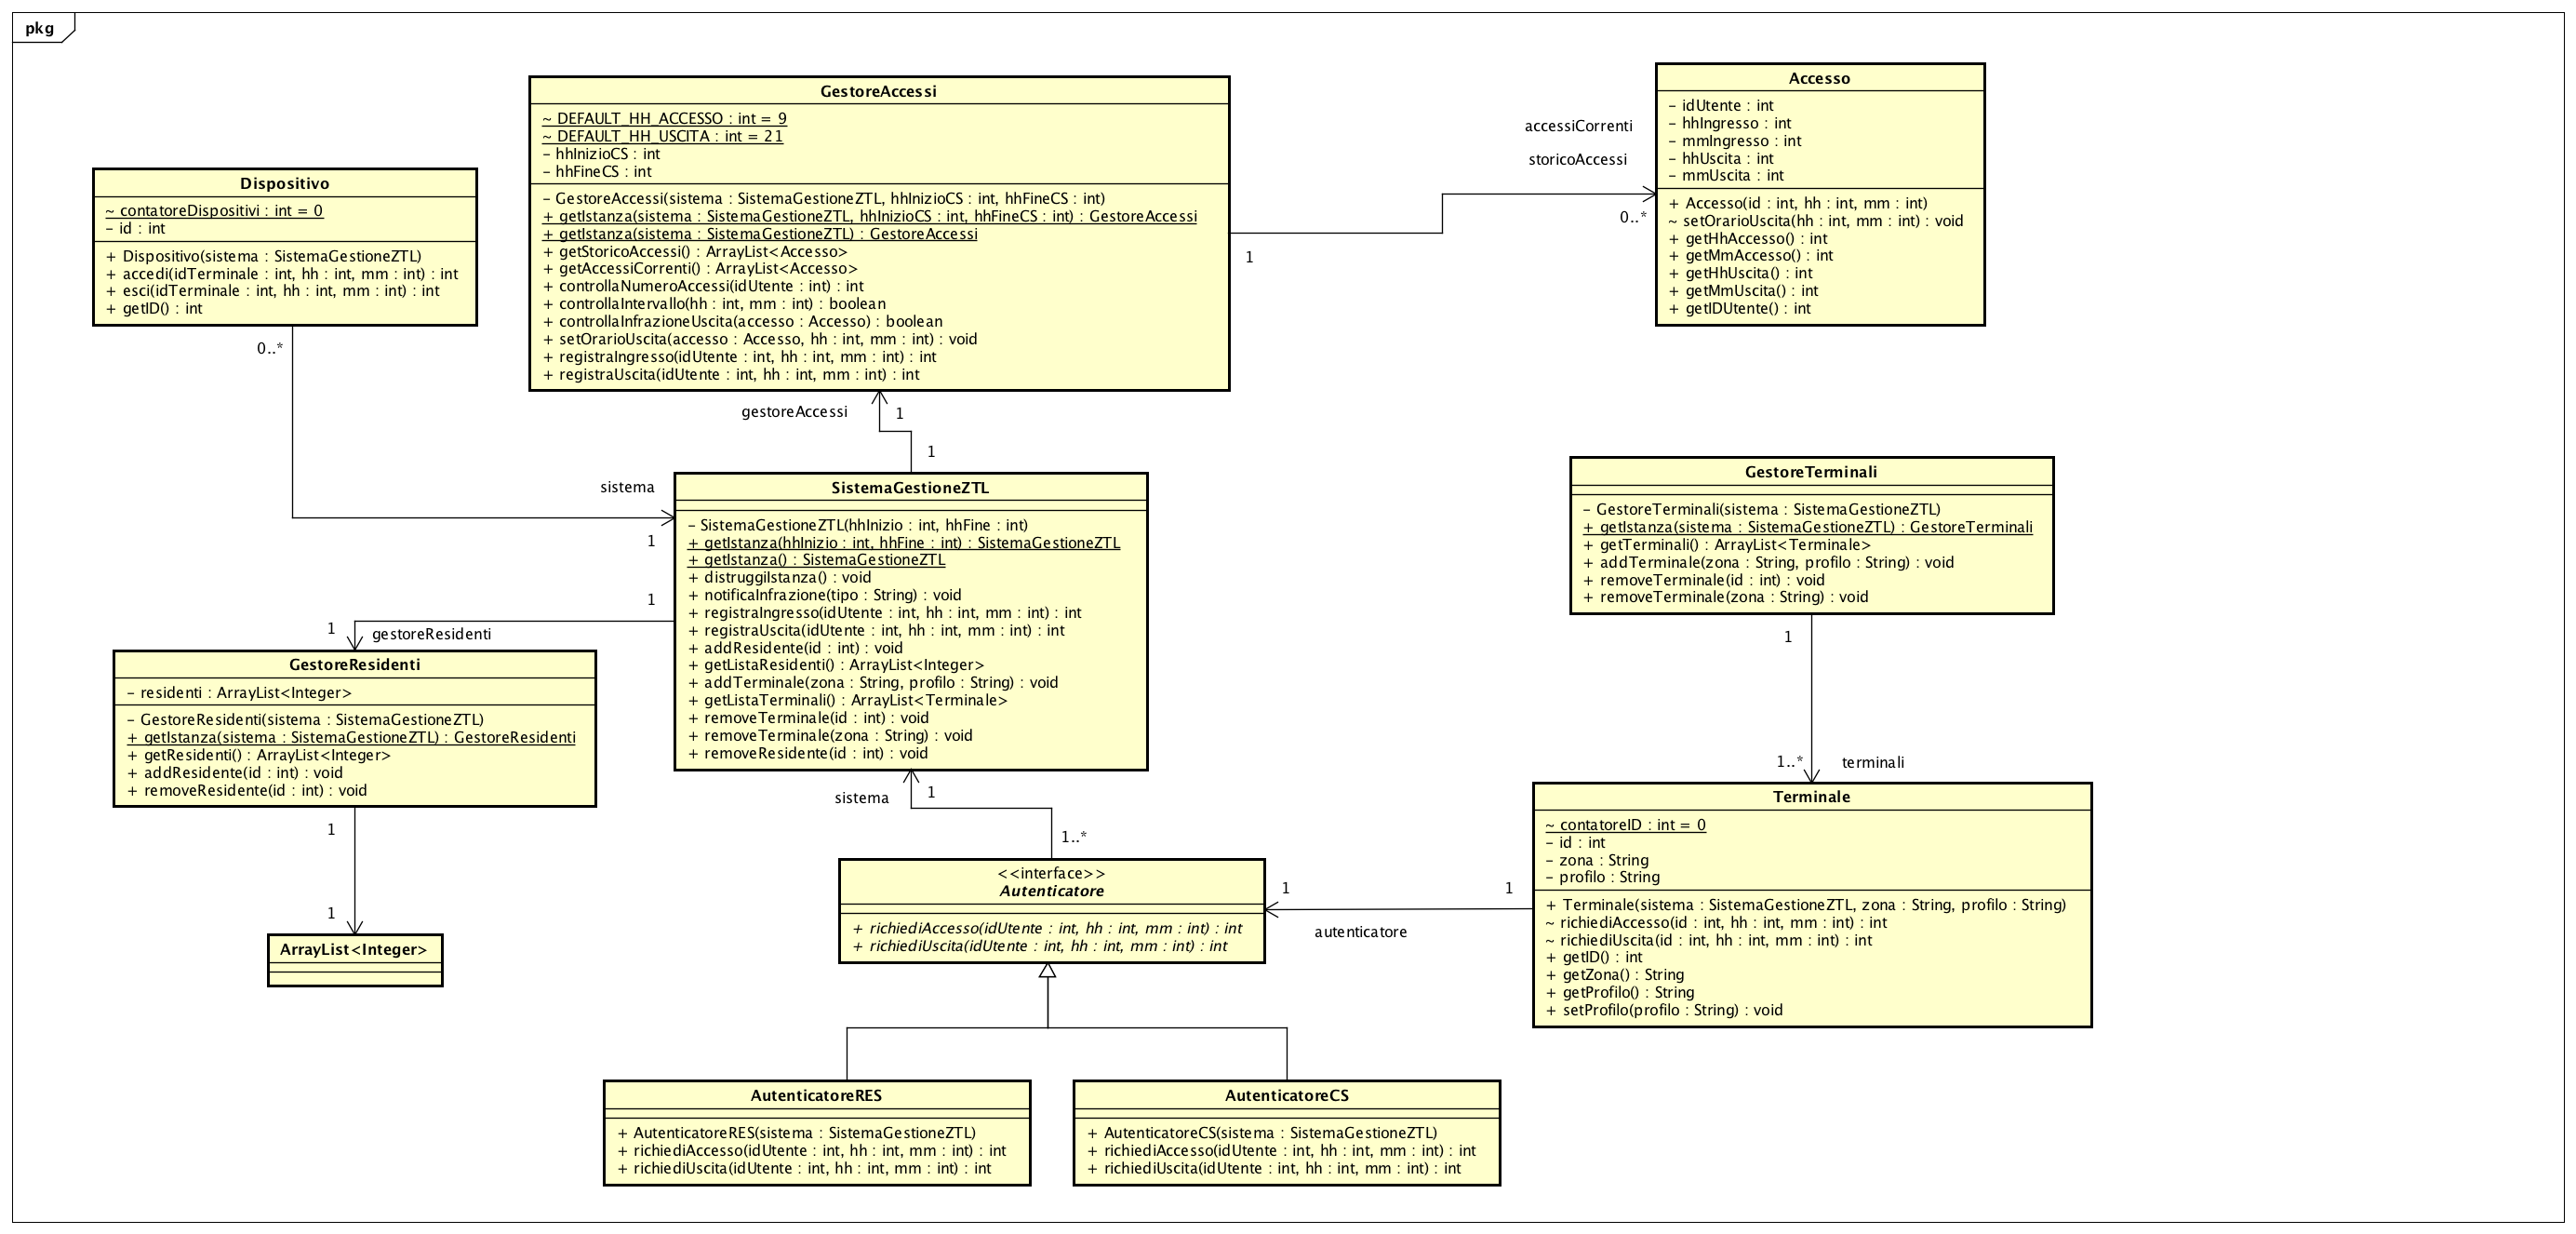
\includegraphics[scale=0.15]{DCD}
    \label{fig:mesh1}
\end{figure}

\section{Motivazioni e Scelte Progettuali}

\subsection{Applicazione Pattern \emph{GRASP} }
Il sistema applica i pattern \emph{GRASP} 
nel seguente modo:
\begin{itemize}
    \item Il sistema centrale è un \emph{Controller}
    in quanto riceve gli input e li delega 
    alle parti del sistema interessate 
    (i gestori, nel nostro caso)
    \item Viene ridotto l'accoppiamento \emph{(Low
    Coupling)} eliminando le dipendenze tra i 
    vari componenti e permettendo comunque una 
    loro comunicazione attraverso il sistema 
    centrale (la classe \emph{SistemaGestioneZTL})
    \item La coesione viene aumentata \emph{(High 
    Cohesion)} grazie alle nuove classi
    \item In particolare, in tal caso, si applica 
    il pattern \emph{Pure Fabrication} dato che 
    le varie classi \emph{gestore} non hanno una 
    controparte reale se non la funzionalità di 
    modularizzare e disaccoppiare il sistema 
    centrale dalle varie mansioni specifiche (di 
    gestire terminali, accessi e quant'altro)
    \item Il pattern \emph{Creator} viene applicato 
    nell'istanziamento degli accessi
    \item L'autenticatore è accoppiato con il sistema 
    centrale, e pertanto leggera i residenti dal 
    \emph{GestoreResidenti} attraverso esso. 
    Peranto abbiamo rimosso il pattern \emph{Observer}
\end{itemize}

\subsection{Applicazione Pattern \emph{GoF}}
I pattern \emph{GoF} sono i seguenti:
\begin{itemize}
    \item Il pattern \emph{Singleton}, non 
    solo per il sistema centrale, ma anche 
    per i vari gestori
    \item Il pattern \emph{Strategy}, per la 
    strategia di autenticazione (per utenti 
    residenti e utenti carico-scarico)
    \item Come ribadito nel precedente paragrafo,
    il pattern \emph{Observer} è stato rimosso 
    in quanto ogni qualvolta un autenticatore 
    necessita di accedere alla lista residenti,
    esso farà una chiamata all'API che il 
    \emph{Sistema Gestione ZTL} fornisce.
    Esso infatti non solo è un controller per 
    l'utente, ma anche per i diversi moduli del 
    sistema
    \item La classe \emph{SistemaGestioneZTL} è
    una potenziale candidata per il pattern 
    \emph{Mediator}, in quanto gia sta assolvendo 
    alla funzione di mediare fra le diverse 
    componenti del sistema, disaccoppiandole.
    Tuttavia per ora non abbiamo fornito un 
    meccanismo per assolvere a tale funzione 
    in maniera standard (aggiungendo/rimuovendo)
    dinamicamente componenti a cui mediare.
\end{itemize}

\section{Casi di Test}

\subsection{Test Unitari}
I test unitari vanno applicati ai metodi
\texttt{controllaNumeroAccessi(), 
controllaIntervallo(), controllaInfrazioneUscita()} 
della classe \emph{GestoreAccessi}. Una volta 
inizializzato il sistema, procediamo ai 
singoli test.

\noindent
Per la funzione \texttt{controllaNumeroAccessi()}
abbiamo:

\begin{enumerate}
    \item Viene fatto accedere un utente una volta.
    Tale utente avrà ID 5 e sarà carico-scarico 
    \item Viene fatto uscire 
    \item Viene chiamato il metodo con il suo ID
    e viene verificato che il valore tornato sia 
    1 (il numero di accessi eseguiti)
    \item Il medesimo metodo viene chiamato con 
    un altro ID utente (1 nel nostro caso). Questo 
    dovrà tornare 0
\end{enumerate}

\noindent
Per la funzione \texttt{controllaIntervallo()}
invece abbiamo il seguente caso di test:

\begin{enumerate}
    \item Viene controllato se l'orario 9:00 
    ricade nell'intervallo, aspettandoci che 
    l'output sia positivo (l'accesso, ricordiamo,
    è permesso dalle 9 alle 21 per gli utenti 
    carico-scarico)
    \item Stessa cosa per l'orario 21:00 (con 
    medesimo risultato)
    \item Viene testato l'orario 8:59 con esito 
    negativo
    \item Viene testato l'orario 21:01 con esito 
    negativo
\end{enumerate}

\noindent
Per la funzione \texttt{controllaInfrazioneUscita()}
invece abbiamo il seguente caso di test:

\begin{enumerate}
    \item Creiamo un accesso che dura dalle 11:00
    alle 12:00. Questo darà \texttt{false}
    \item Creiamo un accesso dalle 11:00 alle 
    12:01. Questo darà \texttt{true}
\end{enumerate}

\subsection{Test unitari per la classe
\texttt{Dispositivo}}
Testiamo i metodi \texttt{accedi()} ed \texttt{esci()}.
In particolare, per il primo:

\begin{itemize}
    \item Istanziamo 4 dispositivi (con ID che varia 
    tra 0 e 3 e nomi d1, d2, d3, d4)
    \item Aggiungiamo due terminali, uno in zona 
    "a" profilo "CS", e l'altro in zona "b" profilo 
    "RES"
\end{itemize}

\noindent
Adesso passiamo al test:

\begin{enumerate}
    \item d1 accede alle 8:59, e questo ritorna -1
    (l'accesso per utenti carico-scarico è dalle 
    9 alle 21)
    \item d2 accede alle 9:00, e questo ritorna 
    1 (l'ID di d2) in quanto in intervallo 
    \item d1 accede, ma questo ritorna 0 in quando 
    d1 è ancora dentro e non può accedere una 
    seconda volta (in tal caso si segna come 0)
    \item d3 accede alle 21, e questo ritorna 
    2 (l'ID di d3)
    \item viene fatto uscire d1 scartando il 
    valore d'uscita (che testeremo nel secondo 
    metodo)
    \item d1 ri-accede alle 15:00, e questo da 
    -1 in quanto ha gia effettuato l'accesso
    \item d4 accede dal terminale RES alle 12,
    questo ritorna -1 in quanto non è residente
    \item d4 diventa residente, e viene fatto 
    accedere due volte, una dal terminale 0 ed 
    una dal terminale 1 (senza uscita). In entrambi 
    i casi viene ritornato l'ID. Questo perchè
    gli utenti residenti non vengono "tracciati",
    ed i loro accessi non vengono registrati
\end{enumerate}

\noindent
Per il secondo metodo:

\begin{itemize}
    \item Istanziamo solo due dispositivi
    \item Aggiungiamo gli stessi terminali del 
    caso di test precedente 
\end{itemize}

\noindent
I passi eseguiti sono i seguenti:

\begin{enumerate}
    \item d1 accede (il risultato viene scartato)
    alle 12:00
    \item d1 esce alle 13, con successo (viene 
    tornato il suo ID) in quanto all'interno dei 
    60 minuti
    \item d1 accede alle 22 (risultato ignorato)
    \item d1 esce alle 22:01, con errore (-1) in 
    quanto fuori intervallo
\end{enumerate}

\subsection{Esecuzione del Test Driver}
Attraverso il test driver, vengono eseguiti 
i test che valutano il sistema nella sua completezza 
a fine iterazione: non testiamo le varie unità,
ma il programma nella sua completezza.
In particolare, queste sono le istruzioni eseguite:
\begin{enumerate}
    \item Inizializzato il sistema con intervallo 
    carico-scarico (9-21)
    \item Creato terminale in zona "a" con profilo CS
    \item Creato terminale in zona "b" con profilo RES 
    \item Aggiunto dispositivo di ID 0
    \item Aggiunto dispositivo di ID 1
    \item Dispositivo di ID 0 diventa residente 
    \item Dispositivo 0 entra alle 7:00 con successo 
    \item Dispositivo 0 esce alle 9:00 con successo
    \item Dispositivo 1 entra alle 10:00 con successo 
    \item Dispositivo 1 esce alle 10:30 con successo 
    \item Dispositivo 1 entra alle 22:00 con due 
    fallimenti: "Ingresso Extra" e "Intervallo 
    Irregolare"
    \item Dispositivo 1 esce alle 20:00, con errore 
    in quanto non esiste accesso attivo associato ad 
    esso
\end{enumerate}

\end{document}